\documentclass[beamer]{standalone}

\usepackage{tikz}

\usetikzlibrary{backgrounds}
\usetikzlibrary{calc}
\usetikzlibrary{positioning}

\definecolor{x-red}{HTML}{e41a1c}
\definecolor{x-blue}{HTML}{3694E0}
\definecolor{x-green}{HTML}{63E05F}
\definecolor{x-purple}{HTML}{D365E3}
\definecolor{x-orange}{HTML}{E8A100}
\definecolor{x-yellow}{HTML}{fff200}

\definecolor{almost-white}{HTML}{fefefe}


\begin{document}

\begin{standaloneframe}


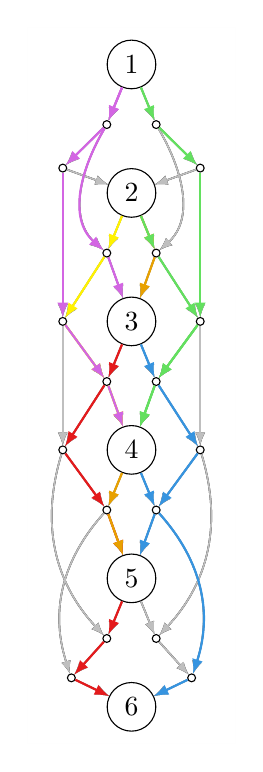
\begin{tikzpicture}[%
        pole/.style={draw, circle, minimum size=.1cm},
        switch/.style={draw, circle, inner sep=0cm, minimum size=.1cm},
        bar/.style={coordinate},
        edge/.style={-latex, lightgray, semithick},
    background rectangle/.style={ draw=almost-white, line width=0pt, },
    show background rectangle,
]

% poles
\node [pole] (p1) at (0,0) {\(1\)};
\node [pole, below=1 of p1] (p2) {\(2\)};
\node [pole, below=1 of p2] (p3) {\(3\)};
\node [pole, below=1 of p3] (p4) {\(4\)};
\node [pole, below=1 of p4] (p5) {\(5\)};
\node [pole, below=1 of p5] (p6) {\(6\)};

\node [switch, below right=.5 and .05 of p1] (s1) {};
\node [switch, below right=.5 and .05 of p2] (s3) {};
\node [switch, right=.5 of p3] (s4) {};
\node [switch] (s2) at ([yshift=-1cm] p1.south -| s4)  {};
\node [switch, below right=.5 and .05 of p3] (s5) {};
\node [switch, right=.5 of p4] (s6) {};
\node [switch, below right=.5 and .05 of p4] (s7) {};
\node [switch, below right=.5 and .05 of p5] (s8) {};
\node [switch, below right=1 and .5 of p5] (s9) {};

\node [switch, below left=.5 and .05 of p1] (r1) {};
\node [switch, below left=.5 and .05 of p2] (r3) {};
\node [switch, left=.5 of p3] (r4) {};
\node [switch] (r2) at ([yshift=-1cm] p1.south -| r4)  {};
\node [switch, below left=.5 and .05 of p3] (r5) {};
\node [switch, left=.5 of p4] (r6) {};
\node [switch, below left=.5 and .05 of p4] (r7) {};
\node [switch, below left=.5 and .05 of p5] (r8) {};
\node [switch, below left=1 and .5 of p5] (r9) {};


% no embedding (black)
\onslide<1>{
    \draw [edge, black] (p1) to (s1);
    \draw [edge, black] (p2) to (s3);
    \draw [edge, black] (p3) to (s5);
    \draw [edge, black] (p4) to (s7);
    \draw [edge, black] (p5) to (s8);

    \draw [edge, black] (s1) to (s2);
    \draw [edge, black, bend left, in=131] (s1) to (s3);
    \draw [edge, black] (s2) to (p2);
    \draw [edge, black] (s2) to (s4);
    \draw [edge, black] (s3) to (p3);
    \draw [edge, black] (s3) to (s4);
    \draw [edge, black] (s4) to (s5);
    \draw [edge, black] (s4) to (s6);
    \draw [edge, black] (s5) to (p4);
    \draw [edge, black] (s5) to (s6);
    \draw [edge, black] (s6) to (s7);
    \draw [edge, black, bend left] (s6) to (s8);
    \draw [edge, black] (s7) to (p5);
    \draw [edge, black, bend left] (s7) to (s9);
    \draw [edge, black] (s8) to (s9);
    \draw [edge, black] (s9) to (p6);


    \draw [edge, black] (p1) to (r1);
    \draw [edge, black] (p2) to (r3);
    \draw [edge, black] (p3) to (r5);
    \draw [edge, black] (p4) to (r7);
    \draw [edge, black] (p5) to (r8);

    \draw [edge, black] (r1) to (r2);
    \draw [edge, black, bend right, in=229] (r1) to (r3);
    \draw [edge, black] (r2) to (p2);
    \draw [edge, black] (r2) to (r4);
    \draw [edge, black] (r3) to (p3);
    \draw [edge, black] (r3) to (r4);
    \draw [edge, black] (r4) to (r5);
    \draw [edge, black] (r4) to (r6);
    \draw [edge, black] (r5) to (p4);
    \draw [edge, black] (r5) to (r6);
    \draw [edge, black] (r6) to (r7);
    \draw [edge, black, bend right] (r6) to (r8);
    \draw [edge, black] (r7) to (p5);
    \draw [edge, black, bend right] (r7) to (r9);
    \draw [edge, black] (r8) to (r9);
    \draw [edge, black] (r9) to (p6);
}

% no embedding (grey)
\onslide<2->{
    \draw [edge] (p1) to (s1);
    \draw [edge] (p2) to (s3);
    \draw [edge] (p3) to (s5);
    \draw [edge] (p4) to (s7);
    \draw [edge] (p5) to (s8);

    \draw [edge] (s1) to (s2);
    \draw [edge, bend left, in=131] (s1) to (s3);
    \draw [edge] (s2) to (p2);
    \draw [edge] (s2) to (s4);
    \draw [edge] (s3) to (p3);
    \draw [edge] (s3) to (s4);
    \draw [edge] (s4) to (s5);
    \draw [edge] (s4) to (s6);
    \draw [edge] (s5) to (p4);
    \draw [edge] (s5) to (s6);
    \draw [edge] (s6) to (s7);
    \draw [edge, bend left] (s6) to (s8);
    \draw [edge] (s7) to (p5);
    \draw [edge, bend left] (s7) to (s9);
    \draw [edge] (s8) to (s9);
    \draw [edge] (s9) to (p6);


    \draw [edge] (p1) to (r1);
    \draw [edge] (p2) to (r3);
    \draw [edge] (p3) to (r5);
    \draw [edge] (p4) to (r7);
    \draw [edge] (p5) to (r8);

    \draw [edge] (r1) to (r2);
    \draw [edge, bend right, in=229] (r1) to (r3);
    \draw [edge] (r2) to (p2);
    \draw [edge] (r2) to (r4);
    \draw [edge] (r3) to (p3);
    \draw [edge] (r3) to (r4);
    \draw [edge] (r4) to (r5);
    \draw [edge] (r4) to (r6);
    \draw [edge] (r5) to (p4);
    \draw [edge] (r5) to (r6);
    \draw [edge] (r6) to (r7);
    \draw [edge, bend right] (r6) to (r8);
    \draw [edge] (r7) to (p5);
    \draw [edge, bend right] (r7) to (r9);
    \draw [edge] (r8) to (r9);
    \draw [edge] (r9) to (p6);
}


% embedding of half adder
\onslide<2>{
\draw [edge, x-green, thick] (p1) to (s1);
\draw [edge, x-orange, thick] (p2) to (s3);
\draw [edge, x-blue, thick] (p4) to (s7);
\draw [edge, x-green, thick] (s1) to (s2);
\draw [edge, x-green, thick] (s2) to (s4);
\draw [edge, x-orange, thick] (s3) to (p3);
\draw [edge, x-green, thick] (s4) to (s5);
\draw [edge, x-green, thick] (s5) to (p4);
\draw [edge, bend left, x-blue, thick] (s7) to (s9);
\draw [edge, x-blue, thick] (s9) to (p6);
\draw [edge, x-purple, thick] (p1) to (r1);
\draw [edge, x-yellow, thick] (p2) to (r3);
\draw [edge, x-red, thick] (p3) to (r5);
\draw [edge, bend right, in=229, x-purple, thick] (r1) to (r3);
\draw [edge, x-purple, thick] (r3) to (p3);
\draw [edge, x-yellow, thick] (r3) to (r4);
\draw [edge, x-yellow, thick] (r4) to (r5);
\draw [edge, x-yellow, thick] (r5) to (p4);
\draw [edge, x-red, thick] (r5) to (r6);
\draw [edge, x-red, thick] (r6) to (r7);
\draw [edge, x-red, thick] (r7) to (p5);
}

% embedding of other graph
\onslide<3>{
\draw [edge, x-green, thick] (p2) to (s3);
\draw [edge, x-blue, thick] (p3) to (s5);
\draw [edge, x-green, thick] (s3) to (s4);
\draw [edge, x-green, thick] (s4) to (s5);
\draw [edge, x-green, thick] (s5) to (p4);
\draw [edge, x-blue, thick] (s5) to (s6);
\draw [edge, x-blue, thick] (s6) to (s7);
\draw [edge, x-blue, thick] (s7) to (p5);


\draw [edge, x-purple, thick] (p1) to (r1);
\draw [edge, x-orange, thick] (p4) to (r7);
\draw [edge, x-red, thick] (p5) to (r8);
\draw [edge, x-purple, thick] (r1) to (r2);
\draw [edge, x-purple, thick] (r2) to (r4);
\draw [edge, x-purple, thick] (r4) to (r5);
\draw [edge, x-purple, thick] (r5) to (p4);
\draw [edge, x-orange, thick] (r7) to (p5);
\draw [edge, x-red, thick] (r8) to (r9);
\draw [edge, x-red, thick] (r9) to (p6);
}



\end{tikzpicture}


\end{standaloneframe}

\end{document}
